\section{Modern cryptography}

\subsection{Composition of ciphers}
So far, we have seen simple historical ciphers and we have discussed how to break them. \textbf{Modern ciphers}, however, are based on very \textbf{simple operations}, such as substitution, XOR, …, that are \textbf{combined} in a smart way so to make the overall algorithm strong and really hard to analyse. It is important to keep in mind that \textbf{combining simple ciphers} does not \textbf{always} \textbf{improve security}. 

For example, consider the shift cipher composed twice. We first shift by $k_1$ and then by $k_2$ modulo 26, as represented in Picture \ref{comp1}.

\begin{figure}[h!]
        \centering
        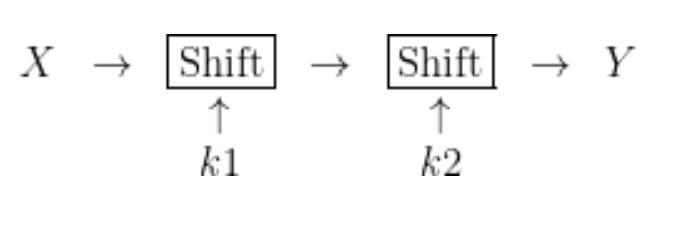
\includegraphics[scale = 1.0]{img/comp1.png}
        \label{comp1}
        \caption{Composition of two shift ciphers - 1}
\end{figure}

It is clear that this is equivalent to shifting by $k_1+k_2$ modulo 26, meaning that applying twice the cipher is the same as applying it once with a key given by the sum of the two keys.

\begin{figure}[h!]
        \centering
        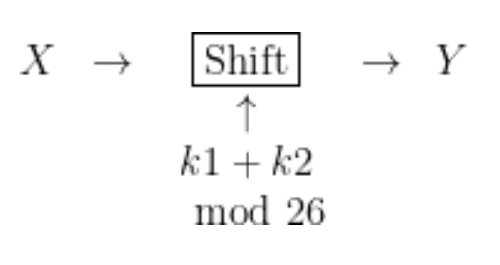
\includegraphics[scale = 1.0]{img/comp2.png}
        \label{comp2}
        \caption{Composition of two shift ciphers - 2}
\end{figure}

This informal reasoning can be made more precise.

\textbf{Definition (Composition)}. We consider two ciphers $S^1=({\cal P}^1,{\cal C}^1,{\cal K}^1,E^1,D^1)$ and $S^2=({\cal P}^2,{\cal C}^2,{\cal K}^2,E^2,D^2)$. We let ${\cal P}^1={\cal C}^1={\cal P}^2={\cal C}^2$, that we note as ${\cal P}$ and ${\cal C}$ in the following. In this way the output of one cipher is for sure a possible plaintext for the second cipher. We can now define \textbf{composition} as $S^1 \times S^2 = ({\cal P},{\cal C},{\cal K}^1\times{\cal K}^2,E,D)$ with

$$
E_{(k1,k2)}(x) = E^2_{k2}(E^1_{k1}(x))
$$

$$
D_{(k1,k2)}(y) = D^1_{k1}(D^2_{k2}(y))
$$

As we can see, in order to encrypt a plaintext $x$ using a composition of two ciphers with keys $k1$ and $k2$ we must:

\begin{enumerate}
    \item \textbf{Encrypt} $x$ using the \textbf{first encryption function} (using $k1$);
    \item \textbf{Encrypt} the \textbf{result} of (1) using the \textbf{second encryption function} (using $k2$).
\end{enumerate}

\example{Consider the composition of the two shifts above. Formally we have that $E^1_k(x) = E^2_k(x) = x+k \mod 26$. Thus,\begin{equation}\begin{align*}E_{(k1,k2)}(x) &= E^2_{k2}(E^1_{k1}(x)) = (x + k1 \mod 26) + k2 \mod 26\\ &= x + (k1+k2 \mod 26) \mod 26 = E^1_{k1+k2 \mod 26}(x)\end{align*}\end{equation}This proves that composing the shift cipher twice is equivalent to applying it once using as a key the sum of the two keys $k1$ and $k2$, modulo 26.}

\subsubsection{Idempotent ciphers}
We have seen that the shift cipher, when repeated twice is equivalent to itself with a different key. When this happens, the cipher $S$ is said to be \textbf{idempotent}, written $S \times S = S$. In this case we know that iterating the cipher will be of no use to improve its security. Even if we repeat it $n$ times we will still get the initial cipher, i.e., $S^n = S$.

We have mentioned that modern ciphers are based on simple operations composed together. Another ingredient is, in fact, \textbf{iteration}. Almost any modern cipher repeats a \textbf{basic core of operations} for a certain number of \textbf{rounds}. It is thus necessary that such core operations do not constitute an idempotent cipher.

It can be proved that if we have two \textbf{idempotent} \textbf{ciphers} that commute, i.e., such that $S^1 \times S^2 = S^2 \times S^1$, then their \textbf{composition} is also \textbf{idempotent}. In this case, we know that iterating their composition is useless. To see why this holds consider one iteration of their composition (recall that function composition is associative):

$$
\begin{array}{ll}(S^1 \times S^2) \times (S^1 \times S^2)\\ = S^1 \times (S^2 \times S^1) \times S^2 &\mbox{ associative property}\\ = S^1 \times (S^1 \times S^2) \times S^2 &\mbox{ commutative property}\\= (S^1 \times S^1) \times (S^2 \times S^2) &\mbox{ associative property}\\ = S^1 \times S^2 &\mbox{ idempotence of the initial ciphers} \end{array}
$$

\subsubsection{Recap}
We have seen examples of how algebraic properties, such as commutativity, can help simplifying the analysis of a cipher. When developing a robust cipher we need to avoid as much as possible that operations can be rearranged, swapped, simplified.

\subsection{The AES cipher}
The \textbf{Advanced Encryption Standard} (AES) has been selected by the National Institute of Standards and Technology (NIST) after a five-year long competition. The original name of the cipher is Rijndael from the names of the two inventors, the cryptographers Joan Daemen and Vincent Rijmen. As any modern cipher, AES is the \textbf{composition} of rather \textbf{simple operations} and contains a \textbf{non-linear component} to \textbf{avoid} \textbf{known-plaintexts attacks} (as the one we have seen on the Hill cipher). The composed operations give a \textbf{non-idempotent cipher} that is \textbf{iterated} for a fixed number of \textbf{rounds} (the longer the key, the more rounds are executed).

Rijndael has been selected because it resulted to be the best one providing:

\begin{itemize}
    \item High \textbf{security} guarantees;
    \item High \textbf{performance};
    \item \textbf{Flexibility} (different key length).
\end{itemize}

All of these \textbf{features} are, in fact, \textbf{crucial} for any modern cipher. Its predecessor, the Data Encryption Standard (DES) is still in use after almost 40 years, in a variant called Triple DES (3DES), which aims at improving the key length. In fact, DES key of only 56 bits is too short to resist brute-forcing on modern, parallel computers.

\subsubsection{Mathematical background}
AES works on the \textbf{Galois Field} with $2^8$ elements noted $\mathbf{GF}(2^8)$. Intuitively, it is the \textbf{set} of all \textbf{8-bit digits} with \textbf{sum} and \textbf{multiplications} performed by interpreting the bits as (binary) \textbf{coefficients of polinomials}. For example, element $11010011$ can be seens as $x^7 + x^6 + x^4 + x + 1$ while $00111010$ is $x^5+x^4+x^3 + x$. The sum will thus be $x^7+x^6+x^4+x+1+x^5+x^4+x^3+x=x^7+x^6+x^5+x^3+1$, since two 1’s coefficient becomes 0, modulo 2, and the term disappears (for example $x + x = 2x = 0x = 0$). We see that \textbf{sum} and \textbf{subtraction} are just the \textbf{bit-wise XOR} of the binary numbers, i.e., $11010011 \oplus 00111010 = 11101001$ which is $x^7+x^6+x^5+x^3+1$.

\textbf{Product} is done \textbf{modulo} the \textbf{irreducible polinomial} $x^8 + x^4 + x^3 + x + 1$. Irreducible means that it cannot be written as the product of two other polinomials (it is, intuitively, the equivalent of primality). 

For example, $(x^7 + x^6 + x^4 + x + 1) \times (x^5+x^4+x^3 + x)$ gives

$$x^{12} + x^{11} + x^9 + x^6 + x^5+x^{11}+x^{10}+x^8+x^5+x^4+x^{10}+x^9+x^7+x^4+x^3+x^8+x^7+x^5+x^2+x$$

, which is reduced to

$$x^{12}+x^6+x^5+x^3+x^2+x$$

Now, the next step is to \textbf{divide} $x^{12}+x^6+x^5+x^3+x^2+x$ by the \textbf{irreducible polynomial} $x^8 + x^4 + x^3 + x + 1$, and find the remainder. In general, long division of polynomials is similar to long division of whole numbers, and when we divide two polynomials we can check the answer using:

$$
\text{dividend} = (\text{quotient} \cdot \text{divisor}) + \text{remainder}
$$

or, equivalently,

$$
\text{dividend} / \text{divisor} = \text{quotient} + \frac{\text{remainder}}{\text{divisor}} 
$$

In our example, dividing $x^{12}+x^6+x^5+x^3+x^2+x$ by $x^8 + x^4 + x^3 + x + 1$ and finding the remainder results as follows:

\begin{enumerate}
    \item Since $x^{12}/x^8 = x^4$, we shift 4 bits to the left the divisor;
    \item Then, we perform a XOR operation between the dividend and the divisor;
    \item Since the results contains 9 bits, which is too much, we perform another XOR operation between the previous result and the divisor;
    \item Finally, we retrieve the remainder, which results to be $11000101$, i.e., $x^7 + x^6 + x^2 + 1$.
\end{enumerate}

$$
\begin{array}{ccccccccccccc}1&0&0&0&0&0&1&1&0&1&1&1&0 \\ 1&0&0&0&1&1&0&1&1 \\\hline & & & &1&1&1&0&1&1&1&1&0\\ & & & &1&0&0&0&1&1&0&1&1 \\\hline & & & & &1&1&0&0&0&1&0&1 \end{array}
$$

This operation is \textbf{quadratic} in general, with respect to the number of bits (8). It can be optimized with the following linear algorithm (which is, in fact, a working python code):

\begin{figure}[h!]
        \centering
        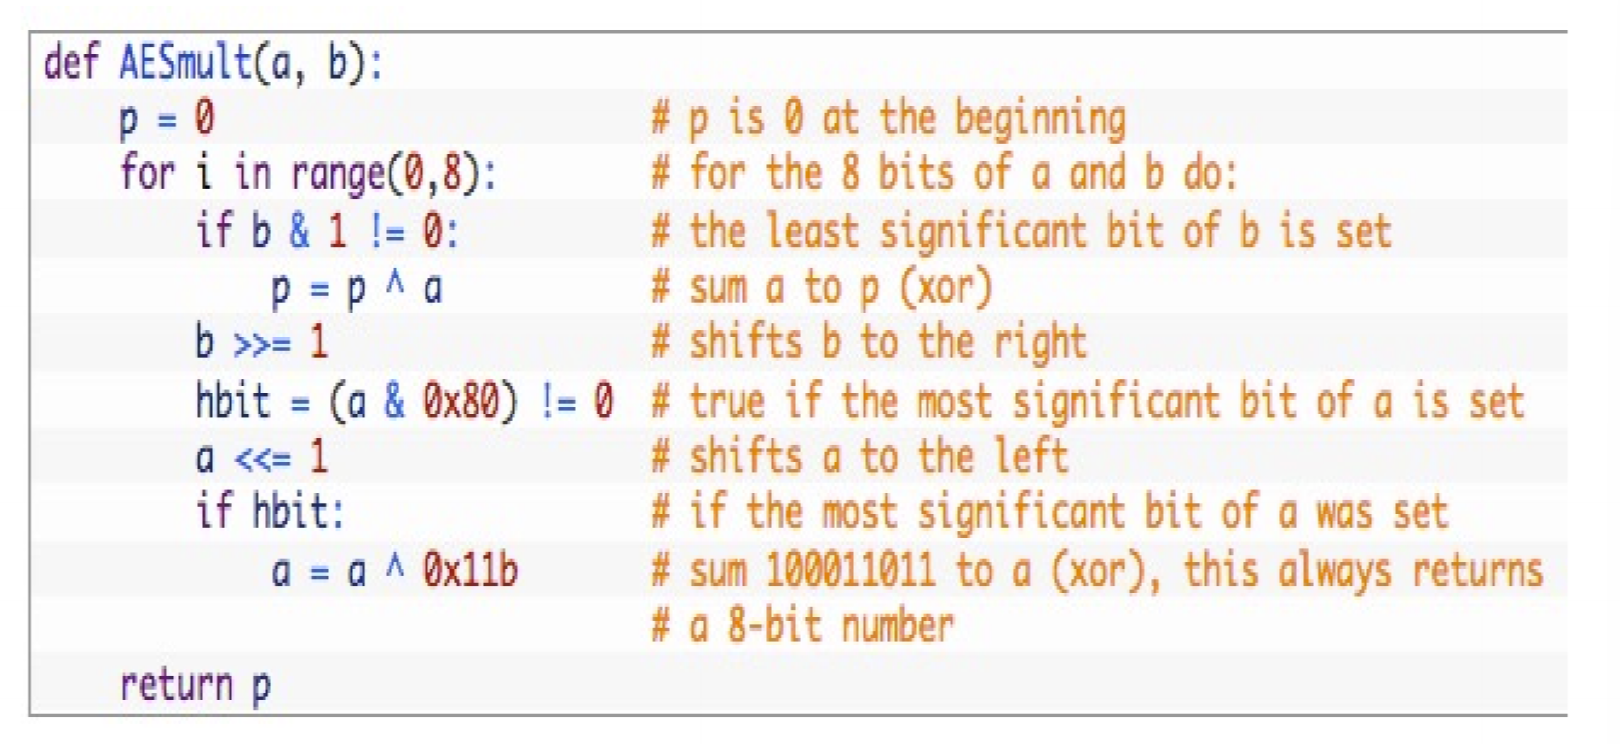
\includegraphics[scale = 0.8]{img/aes1.png}
        \label{aes1}
        \caption{Product - optimization}
\end{figure}

The \textbf{optimization} works as follows:

\begin{enumerate}
    \item We let $a$ to be the binary representation of the coefficients of the first term of the multiplication, and $b$ the binary representation of the coefficients of the second one;
    \item We let $p = 00$;
    \item We perform a XOR operation between $a$ and $p$, and we update $p$ with the result of this operation;
    \item Then, $b$ is shifted to the right and $a$ is shifted to the left meaning that we respectively divide and multiply by $x$ the two polynomials. Now we erase the least significant bit of $b$ and we add a 0 to $a$:
    \begin{itemize}
        \item If the least significant bit is a 1, we continue performing the XOR operation between the new $a$ and $p$;
        \item Otherwise, we skip the XOR operation. 
    \end{itemize}
    \item When $a$ becomes more than $2^8$ we need to XOR to it the modulus $100011011$, i.e. $0x11b$, to keep it 8-bits long.
\end{enumerate}

An example is provided in Picture \ref{aes8}.

\begin{figure}[h!]
        \centering
        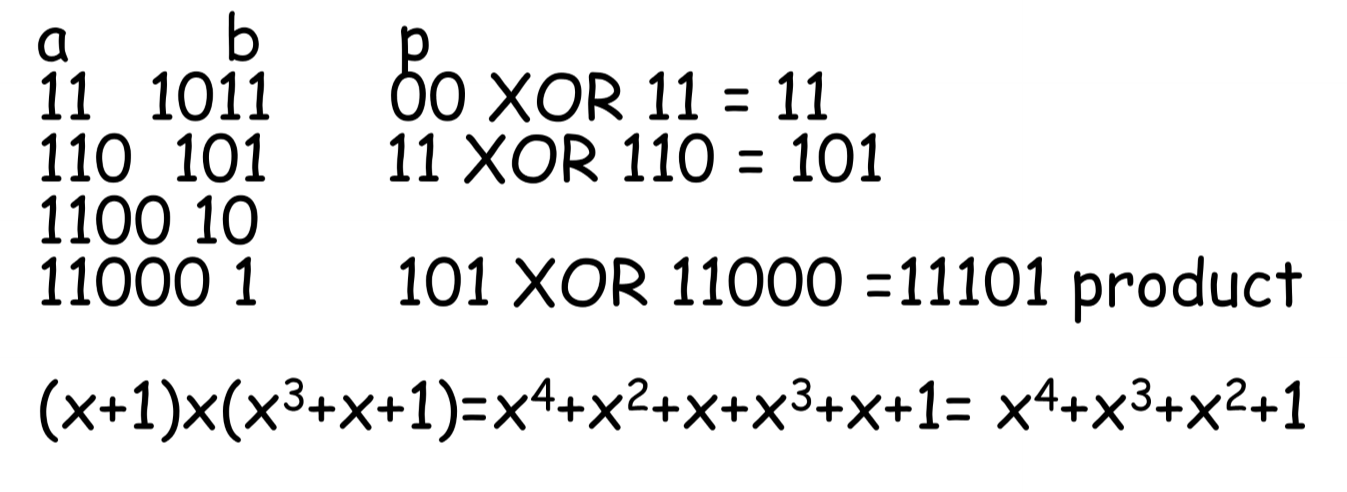
\includegraphics[scale = 0.65]{img/aes8.png}
        \label{aes8}
        \caption{Product - optimization: example}
\end{figure}

The \textbf{correctness} of this algorithm derives from the \textbf{invariant} which states that after each loop: 

\begin{itemize}
    \item $ab+p$ is the product of the initial $a$ and $b$ (all operation does in the Galois Field);
    \item Since $b$ is 0 at the end, we have that $p$ will contain the product.
\end{itemize}

\subsubsection{The AES cipher}
Now that we have introduced the basic operation used to implement AES we can describe the cipher. The official \textbf{description} of \textbf{AES} is available on-line.

AES operates on a \textbf{4×4 matrix} of bytes. We have that 16 bytes are 128 bits which is, in fact, the block size. \textbf{Plaintext} bytes $b_1,\ldots,b_{16}$ are copied in the matrix by columns following this scheme:

$$  \begin{bmatrix}b_1&b_5&b_9&b_{13}\\b_2&b_6&b_{10}&b_{14}\\b_{3}&b_7&b_{11}&b_{15}\\b_4&b_8&b_{12}&b_{16}
    \end{bmatrix}
$$

Cipher \textbf{keys} have lengths of 128, 192, and 256 bits. AES has \textbf{10 rounds} for 128-bit keys, \textbf{12 rounds} for 192-bit keys, and \textbf{14 rounds} for 256-bit keys. Rijndael was designed to handle additional block sizes and key lengths, however they are not adopted in the AES standard. A round is composed of different operations, all of which are invertible:

\begin{enumerate}
    \item \textbf{AddRoundKey}: the round \textbf{key} (see Key Expansion, below) is bitwise \textbf{XOR}-ed with the \textbf{block}. A round key is thus 128 bits, independently of the chosen key size.

    \begin{figure}[h!]
        \centering
        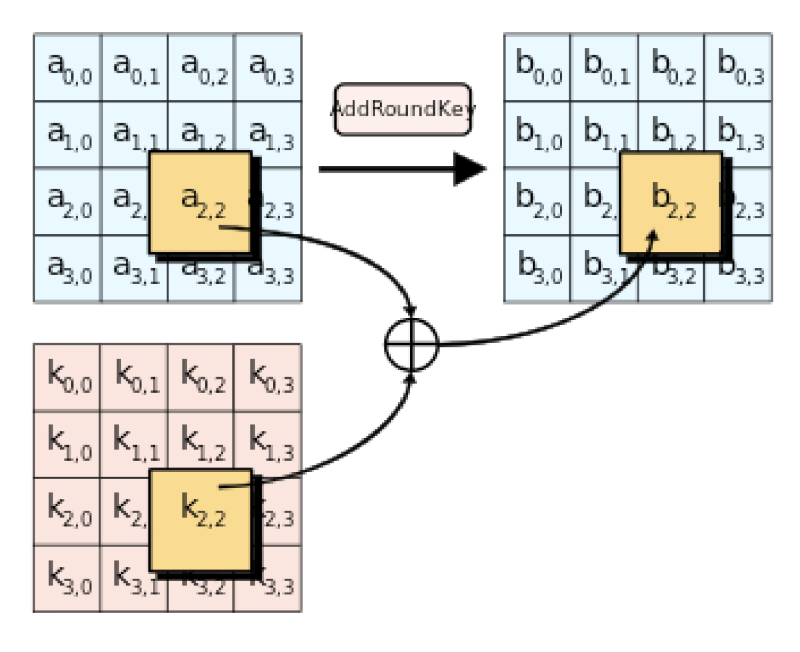
\includegraphics[scale = 0.8]{img/aes2.png}
        \label{aes2}
        \caption{AddRoundKey operation}
    \end{figure}

    In this example, $b_{2,2} = a_{2,2} \text{ XOR } k_{2,2}$.
    
    \item \textbf{SubBytes}: a \textbf{fixed }\textbf{non-linear substitution}, called \textbf{S-box}, is applied to each byte of the block. The substitution is reported below. Given a \textbf{byte} in hexadecimal notation, the \textbf{first digit} is used to select a \textbf{row} and the \textbf{second} one to select a \textbf{column}. For example, $0x25$ would be the third row (2) and the sixth column (5) giving $0x3f$.

    \begin{figure}[h!]
        \centering
        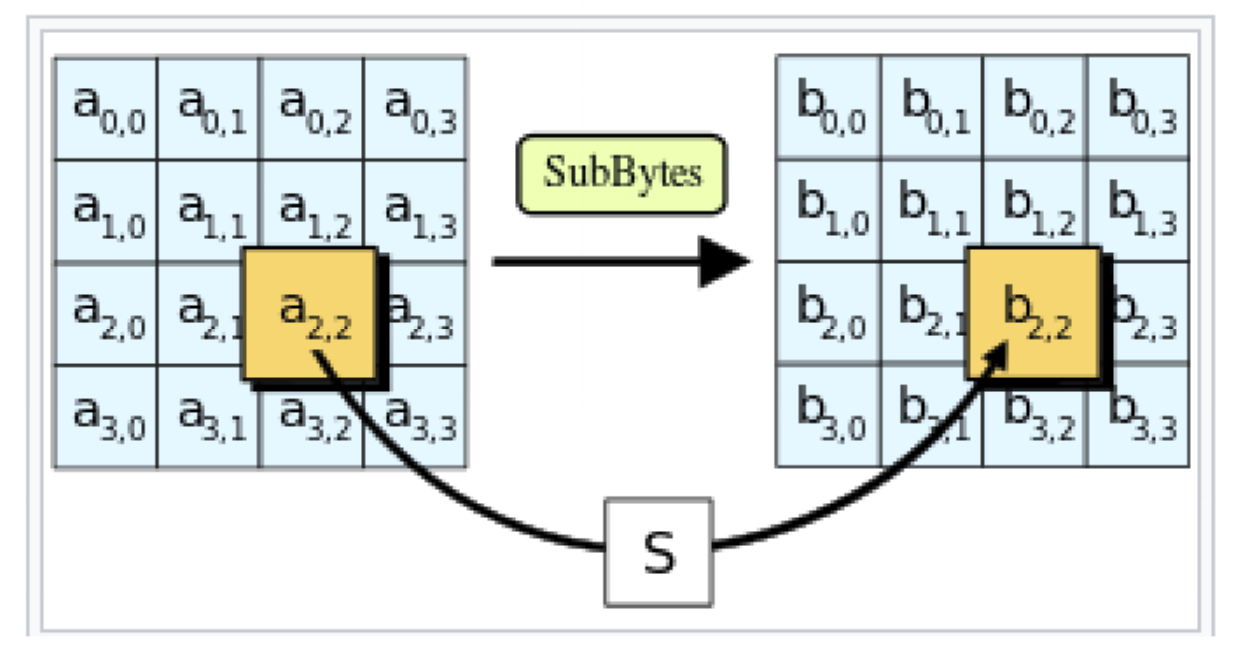
\includegraphics[scale = 0.65]{img/aes3.png}
        \label{aes2}
        \caption{SubBytes operation}
    \end{figure}

    The S-box is represented below:

    \begin{figure}[h!]
        \centering
        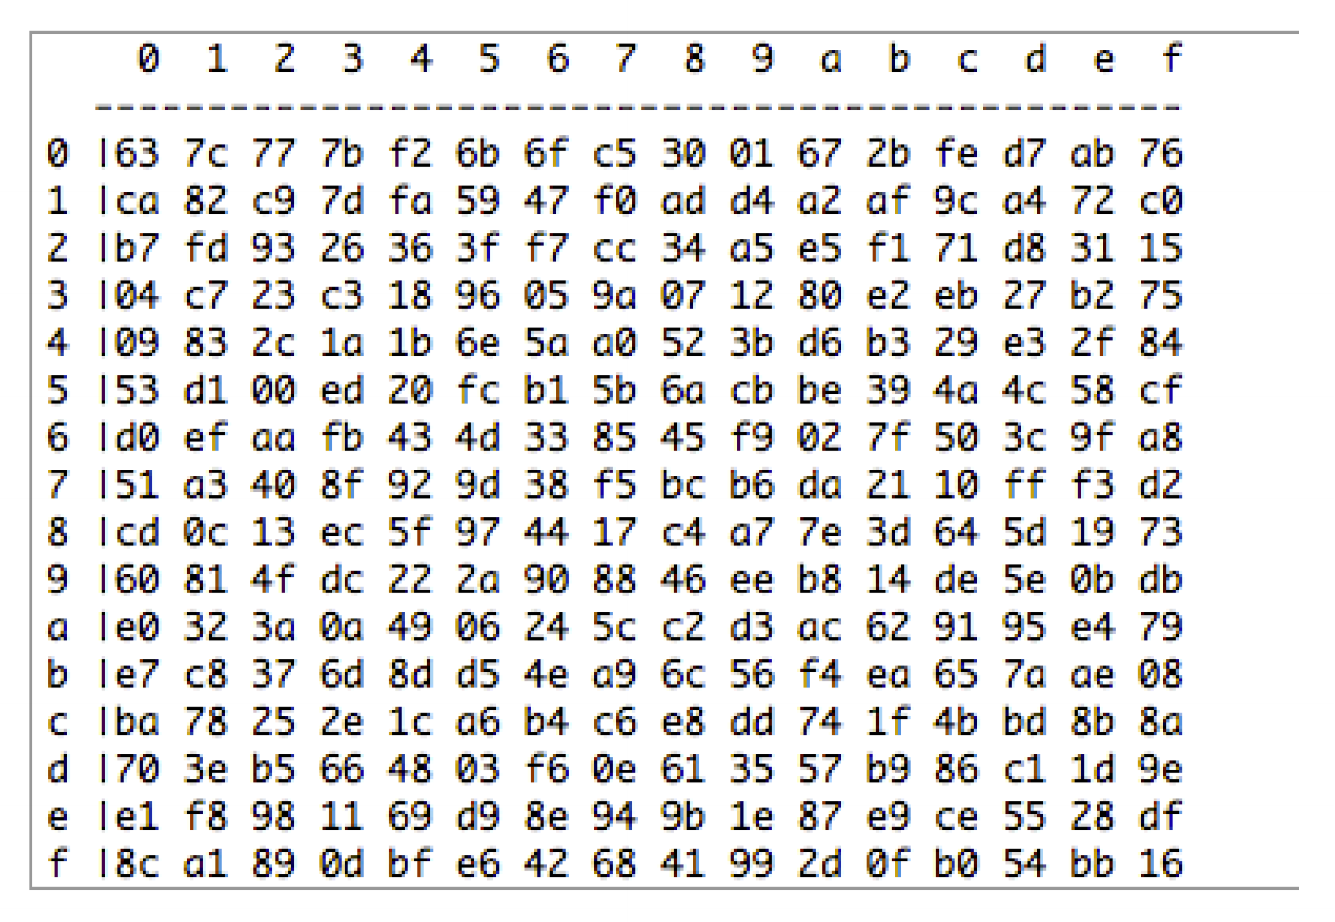
\includegraphics[scale = 0.8]{img/aes4.png}
        \label{aes4}
        \caption{S-box}
    \end{figure}

    Notice that S-box is secure because the attacker cannot easily retrieve $b_{2,2}$, since $2^{16}$ possible values exist. Moreover, this S-box has been obtained by taking, for each byte, its \textbf{multiplicative inverse} in the finite field (that can be computed efficiently via an algorithm that we will see later on), noted $b_7, \ldots, b_0$, and applying the affine transformation $b_i = b_i \oplus b_{i+4 \mod 8} \oplus b_{i+5 \mod 8} \oplus b_{i+6 \mod 8}\oplus b_{i+7 \mod 8} \oplus c_i$, with $c_i$ representing the i-th bit of $01100011$. The above transformation can be written as:

    \begin{figure}[h!]
        \centering
        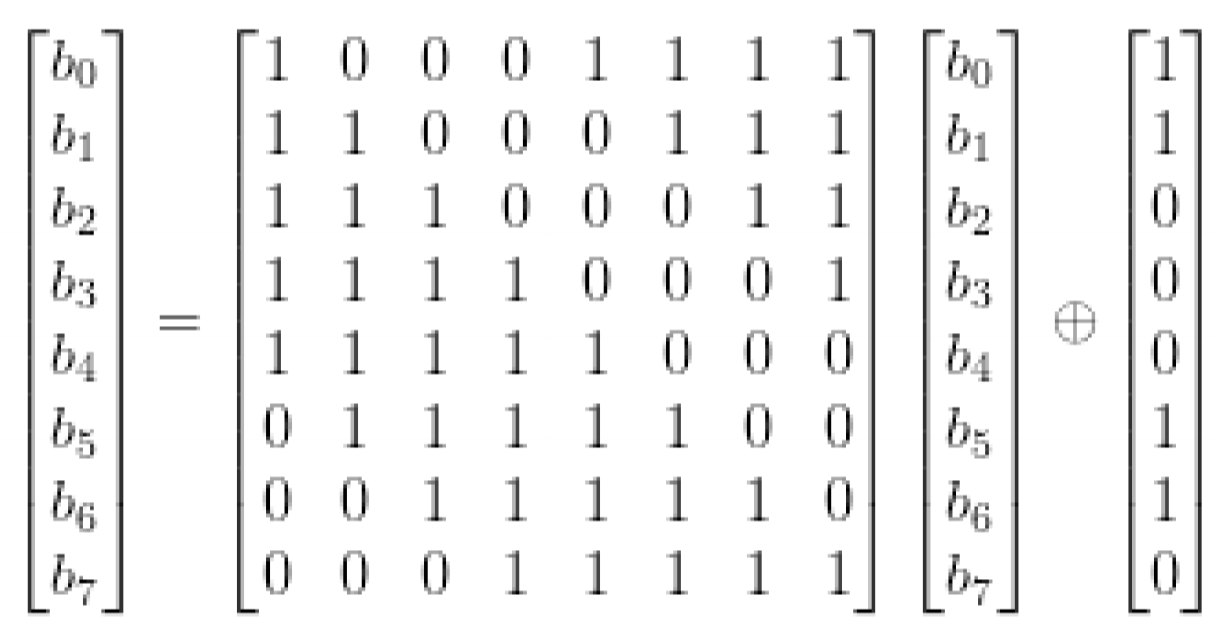
\includegraphics[scale = 0.65]{img/aes5.png}
        \label{aes5}
        \caption{Generation of the S-box}
    \end{figure}

    Using multiplicative inverses is known to give \textbf{non-linear properties}, while the affine transformation complicates the attempt of algebraic reductions.

    \item \textbf{ShiftRows}: \textbf{rows} of the block matrix are \textbf{shifted} to the left by 0,1,2,3, respectively. The shift is circular:

    \begin{figure}[h!]
        \centering
        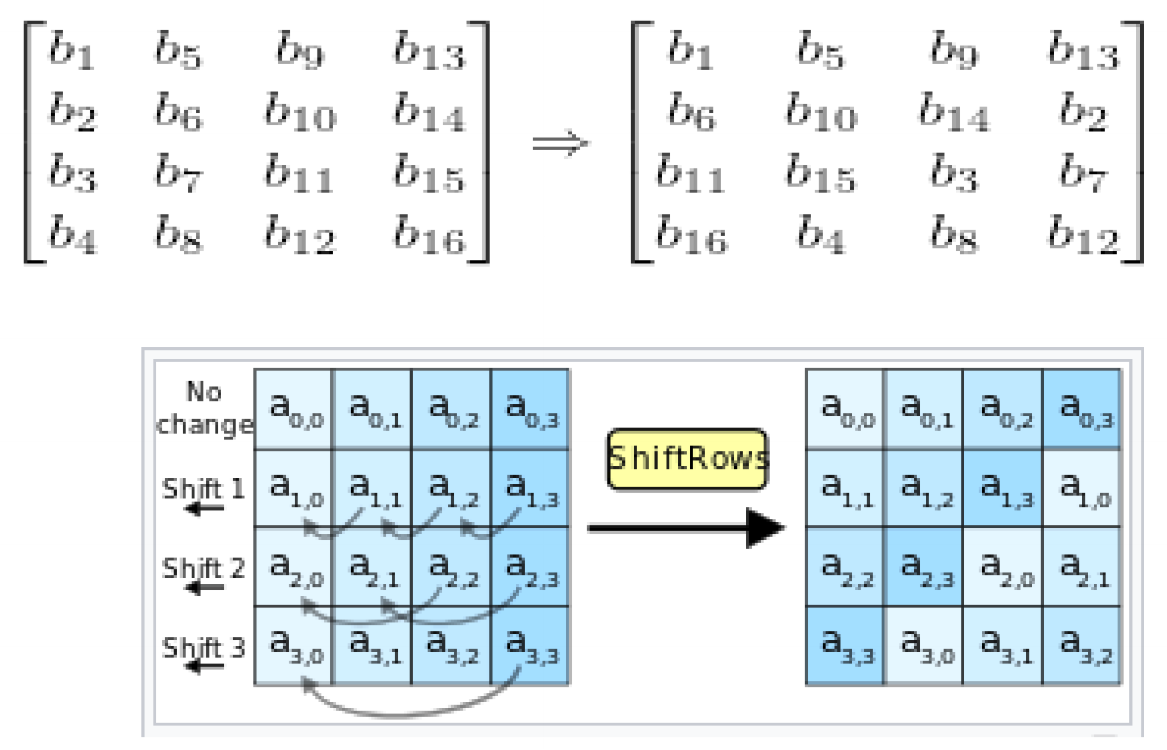
\includegraphics[scale = 0.8]{img/aes6.png}
        \label{aes6}
        \caption{ShiftRows operation}
    \end{figure}

    \item \textbf{MixColumns}: columns of the block matrix are multiplied by the following matrix:

    \begin{figure}[h!]
        \centering
        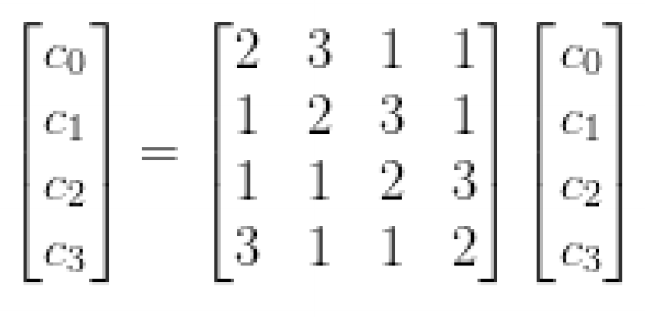
\includegraphics[scale = 0.8]{img/aes7.png}
        \label{aes7}
        \caption{MixColumns operation}
    \end{figure}

    For example the first byte of each column is computed as $2c_0 \oplus 3c_1 \oplus c_2 \oplus c_3$.

    \underline{NOTE}: this fixed matrix is obtained by considering each column as a four-term polynomial with coefficients in $\mathbf{GF}(2^8)$. The columns are then multiplied modulo $x^4 + 1$ with a fixed polynomial $a(x)$, given by $a(x) = 3x^3 + x^2 + x + 2$. This specific modulus is such that, e.g., $x^4$ becomes $x^0$, $x^5$ becomes $x^1$ and so on..

    \item \textbf{Key Expansion} (not covered during the lecture): we have mentioned that AES uses round keys in the AddRoundKey step. These keys are in fact derived from the initial AES key as follows. 
    
    \textbf{Keys} are represented as \textbf{arrays of words} of 4 bytes. So, for example, a 128 bit key will be 4 words of 4 bytes, i.e., 16 bytes. This is expanded into an array of size $4 * (N_r + 1)$, where $N_r$ is the \textbf{number of rounds}. In this way we obtain 4 different words of key for each round.
    
    Let $N_k$ note the \textbf{number of words} of the \textbf{initial key} (e.g. 4 for 128 bits). The first $N_k$ words of the key array are the same as the initial key. Next $i$-th word is obtained from the previous $i-1$ word, possibly transformed as described below, XOR-ed with word $i$-$N_k$. The transformation happens only for words in position multiple of $N_k$ and consists of a cyclic left shift of word bytes by one position (\textit{RotWord}) followed by a byte-wise application of the S-box (\textit{SubWord}) and a XOR with a round constant (\textit{Rcon}). This constant at step $j$ is the word $[x^{j-1},0x00,0x00,0x00]$ with $x^{j-1}$ computed in the Galois field, meaning $02^{j-1}$ since polynomial $x$ is the binary number $00000010$, i.e., $0x02$.

    The pseudocode for this phase is represented Picture \ref{aes9}.

    \begin{figure}[h!]
        \centering
        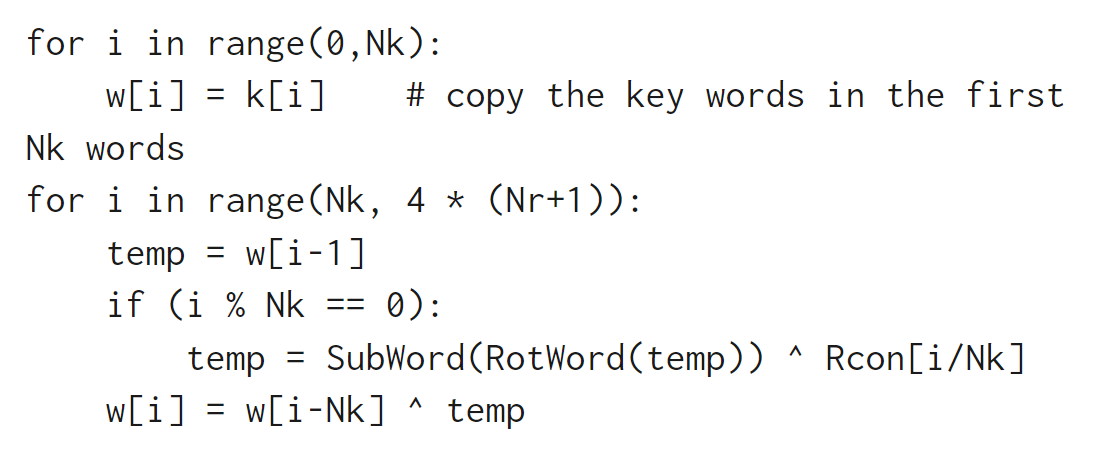
\includegraphics[scale = 0.8]{img/aes9.png}
        \label{aes9}
        \caption{Key Expansion operation}
    \end{figure}

    IMPORTANT NOTE: for 256 bit key, when i-4 is a multiple of $N_k$ \textit{SubWord} is applied to $w[i-1]$ before the XOR. This has been omitted in the code for the sake of readability. Moreover, note that of course the first byte of \textit{Rcon} can be precomputed.

\end{enumerate}

Here is the \textbf{overall scheme} for AES assuming that variable state is initialized with the 4x4 matrix of the plaintext (see above) and $w[]$ has been initialized by key expansion.

\imageLabel{img/aes10.png}{0.8}{Scheme of AES - Encryption}{aes10}

Notice that in the \textbf{last round we do not perform} the \textit{MixColumn} \textbf{operation}.

\textbf{Decryption} is computed by \textbf{applying inverse operations}.

\imageLabel{img/aes11.png}{0.8}{Scheme of AES - Decryption}{aes11}

Notice that:

\begin{enumerate}
    \item \textit{AddRoundKey} is unchanged since XOR is the inverse of itself;
    \item \textit{InvShiftRows} trivially amounts to revert the shifts on the row (to the right instead of left);
    \item \textit{InvSubBytes} is computed by using the following inverse substitution of the S-Box:

    \imageLabel{img/aes12.png}{0.8}{Inverse S-Box}{aes12}

    \item Finally, \textit{InvMixColumns} is given by the following operation:

    \imageB{img/aes13.png}{0.8}

    For example the first byte of each column is computed as $0e c_0 \oplus 0b c_1 \oplus 0d c_2 \oplus 09 c_3$.

    \textbf{NOTE}: this fixed matrix is obtained by considering each column as a four-term polynomial with coefficients in $\mathbf{GF}(2^8)$. The columns are then multiplied modulo $x^4 + 1$ with the inverse of the fixed polynomial $a(x)$, given by $a^{-1}(x) = 0b x^3 + 0d x^2 + 09 x + 0e$.
    
\end{enumerate}

The algorithm for decryption is written in a form similar to the one for encryption but operations are not in the same order. It can, in fact, become the very same algorithm by noticing that:

\begin{enumerate}
    \item \textit{SubBytes} and \textit{ShiftRows} commute. It does not matter if we first apply the byte-wise substitution or if we first shift the rows. The final result will be the same. Of course, the same holds for the inverse transformations;

    \item \textit{InvMixColumns}$(\text{state} \oplus \text{roundKey})$ = \textit{InvMixColumns}(\textit{state}) $\oplus$ \textit{InvMixColumns}(\textit{roundKey}). This allows for inverting the two functions, provided that \textit{InvMixColumns} is applied to the all the round keys.

\end{enumerate}

Call $dw$ the array containing the round keys transformed via InvMixColumns. The final decryption algorithm is represented in Picture \ref{aes16}.

\imageLabel{img/aes16.png}{0.8}{Decryption algorithm}{aes16}

This is exactly the same as the one for encryption, but with the inverse functions. Having the same algorithm for encryption and decryption simplifies a lot implementations, especially if they are done in hardware.

The final scheme of the AES algorithm is provided in Picture \ref{aes14}: note that AES is a symmetric key algorithm.

\imageLabel{img/aes14.png}{0.8}{AES algorithm}{aes14}

Finally, we recall the fact that the security of AES depends on the number of rounds that are executed: the more rounds, the more secure the algorithm is.

\subsection{Block cipher modes of operation}
When using block ciphers we have to face the problem of encrypting \textbf{plaintexts} that are \textbf{longer} than the \textbf{block size}. We then adopt a \textbf{mode of operation}, i.e., a \textbf{scheme} that repeatedly applies the \textbf{block cipher} and allows for encrypting a plaintext of arbitrary size.

\subsubsection{Electronic CodeBlock mode (ECB)}
This is the simplest mode and is, in fact, what we have done so far with classic ciphers: the \textbf{plaintext} $X$ is split into \textbf{blocks} $x_1,x_2,\ldots,x_n$ whose \textbf{size} is exactly the same as the size of the \textbf{cipher block}. Each \textbf{block} is then \textbf{encrypted} independently using the fixed \textbf{key} $k$. For example, a substitution cipher applies to letters. What we do is to split the plaintext into single letters that are encrypted independently.

\image{img/bcm1.png}{0.90}{ECB: Encryption}

\textbf{Decryption} is done, as expected, by reversing the scheme:

\image{img/bcm2.png}{0.90}{ECB: Decryption}

\underline{\textbf{Advantage}}: this scheme has the advantage of being very \textbf{simple} and \textbf{fast}, especially on \textbf{multi-core computers}. Notice, in fact, that each single encryption/decryption can be performed \textbf{independently}.

\underline{\textbf{Disadvantages}}: the \textbf{security} of the scheme, however, is \textbf{poor}. Indeed:

\begin{enumerate}
    \item It mainly conveys all the \textbf{defects} of \textbf{monoalphabetic classic ciphers}: equal plaintext blocks are encrypted in the same way. This allows for the construction of a code-book (from which the mode name) mapping ciphertexts back to plaintexts. It is often the case, in practice, that part of a plaintext is fixed due to the message format, for example. Think of a mail starting with “Dear Alice, …”. If we know a part of the plaintext, we know how the blocks containing that part are encrypted. We can use this information to decrypt other parts of the message, whenever we see the same block occurring.

    Picture \ref{bcm5} provides an immediate visualization of the codebook problem described above.

    \imageLabel{img/bcm5.png}{0.8}{Attack on ECB}{bcm5}

    \item Another crucial limitation of this mode is the complete \textbf{absence of integrity}: an \textbf{attacker} in the middle might duplicate, swap, eliminate encrypted blocks and this would correspond to a plaintext where the same blocks are duplicated, swapped, eliminated. Again, having information about the format of the plaintext, an attacker might be able to obtain a different meaningful plaintext. How critical is this attack really depends on the application. But it is not a good idea to leave such an easy opportunity.
    
\end{enumerate}

\subsubsection{Cipher Block Chaining mode (CBC)}
This mode solves or mitigates all the issues of ECB discussed above: it \textbf{prevents} \textbf{equal plaintexts} to be \textbf{encrypted} the \textbf{same way} and, at the same time, it provides a \textbf{higher degree of integrity}, even if it is not yet satisfactory on this aspect. The idea is to \textbf{“chain” encryption of blocks} using the \textbf{previous encrypted block}. The first block is chained with a special number called \textit{Initialization Vector} (\textit{IV}) that is kept secret together with key $k$.

\image{img/bcm3.png}{0.90}{CBC: Encryption}

\textbf{Decryption} is as follows:

\image{img/bcm4.png}{0.90}{CBC: Decryption}

\underline{\textbf{Advantage}}: as mentioned above, \textbf{CBC} \textbf{never encrypts the same plaintext block in the same way}, preventing the code-book attack. \textbf{Integrity} is improved, but is not yet completely satisfactory. If an attacker swaps, duplicates or eliminates encrypted blocks this will result in at least one corrupted plaintext block. Notice however that this might be unnoticed at the application level and, again, we cannot leave to the application the whole task of checking integrity of decrypted messages.

\underline{\textbf{Disadvantage}}: using \textbf{XOR} introduces a \textbf{new weakness}: the \textbf{attacker} manipulating \textbf{one bit} of an \textbf{encrypted block} $y_i$ obtains that the \textbf{same bit of plaintext} $x_{i+1}$ is also \textbf{manipulated}. At the same time $x_i$ is corrupted.

\subsubsection{Output FeedBack mode (OFB)}
We now see two modes of operation that “transform” block ciphers into stream ciphers. The general idea is to use the block cipher to generate a complex key stream. Encryption is then performed by just XOR-ing the plaintext blocks with the keys of the stream. Intuitively, this is like one-time-pad with a generated key stream. The more the stream is close to a random stream the more the cipher will be close to a perfect one.

\image{img/bcm6.png}{0.90}{OFB: Encryption}

Notice that key generation is completely independent of the plaintext and ciphertext. In fact, it is possible to generate the key stream offline, having key k, and perform encryption later on, when necessary. Decryption simply consists of “swapping the arrows” when performing the XOR: ciphertexts are XOR-ed with the key stream to recover the plaintexts.

\image{img/bcm7.png}{0.90}{OFB: Decryption}

Notice that the generation of the key stream is, in fact, CBC encryption of a zero plaintext (indeed, notice that in this case we do not have the top level $x_i$ XOR $y_{i-1}$). It is thus possible to reuse CBC implementations to compute it. Notice also that the plaintext blocks can be smaller that the size of the block cipher. In that case it is possible to use part of the key and use the remaining part for the next block. For example, if the size of the block is 128 bits (like in AES), and we have to encrypt single bytes we have that one key can be split into $128/8 = 16$ keys of 8 bits, each used to encrypt a single byte.

\underline{\textbf{Advantages}} 

\begin{itemize}
    \item This cipher is very efficient (key can be precomputed using CBC) and allows for the encryption of streams of plaintexts;
    \item Key stream is generated through a block cipher which makes it very hard to be predicted;
    \item Finally, notice that it works very well when IV changes every time we encrypt a new block.
\end{itemize}

\underline{\textbf{Disdvantages}} 

\begin{itemize}
    \item This stream cipher is synchronous since the key stream is independent of the plaintext. As a consequence, if we reuse the same IV with the same key we obtain the same key stream. Since encryption is XOR, attacking the cipher is the same as attacking one-time-pad when the key is used more than once. Thus, the IV must be changed any time we encrypt a new message under the same key k;
    \item Moreover, an attacker in the middle can arbitrarily manipulate bits of the plaintext by swapping the corresponding bits in the ciphertext. No decrypted blocks will be corrupted. For this reason this mode should only be used in application where integrity of the exchanged message is not an issue or is achieved via additional mechanisms. An example could be satellite transmissions where an attacker is extremely unlikely to be in the middle and confidentiality is the only issue. In this setting, absence of integrity becomes useful to avoid noise propagation: an error on one bit will only affect one bit of the plaintext.
\end{itemize}

\underline{NOTE}: there exists a variation of OFB, called \textbf{Counter mode} (\textbf{CTR}), where IV is a random number (nounce) and a counter. The random number can be sent in clear (the bit should change and any new stream generation), and the counter changes the value during the stream generation. This mode is widely used in practice.

\image{img/bcm10.png}{1.8}{CTR: Encryption}

\subsubsection{Cipher FeedBack mode (CFB)}
This mode mitigates the problems of OFB by making the key stream dependent on the previous encrypted element. To preserve the ability of encrypting plaintexts of size less than or equal to the size of the block of the cipher (e.g. a single byte), this mode uses a shift register that is updated at each step: the register is shifted to the left the number of bits of previous ciphertext (8 for a byte), and such a ciphertext is copied into the rightmost bits of the register.

\image{img/bcm8.png}{0.90}{CFB: Encryption}

In this sense, in the first phase we use IV, and in the following ones we use blocks of the previous outputs ($\text{IV}|y_1$ or $y_{n-2}|y_{n-1}$). Decryption is as follows:

\image{img/bcm9.png}{0.90}{CFB: Decryption}

As for OFB, the key stream is generated and then XOR-ed to the ciphertexts to reconstruct the plaintexts.

\underline{\textbf{Advantage}}: this mode provides a higher degree of integrity with respect to OFB: whenever one bit of one ciphertext is modified, the next BSize/CSize plaintexts are corrupted, where BSize is the size of the block of the cipher (e.g., 128 bites) and CSize is the size of the single ciphertext (e.g., 8 bits). For example, with AES and 8 bits of plaintext/ciphertext sizes, we have $128/8 = 16$ corrupted decryptions. This number corresponds to the number of left shifts necessary for a ciphertext to exit the shift register. 

\underline{\textbf{Disadvantage}}: on the other hand, this cipher is slower than OFB as it requires the previous ciphertext to compute the next, meaning that parallelization is impossible when encrypting. Moreover, for noisy transmissions (e.g., satellite, TV, ..) it has the problem of propagating an error on a single bit over the next BSize/CSize plaintexts, which are completely corrupted.

\subsection{More block ciphers}
There are many other ciphers in use, in addition to AES. We list some here giving a very brief summary of their features.

\subsubsection{Data Encryption Standard (DES)}
This is the predecessor of AES. It has been published in 1975 and derives from Lucifer (IBM). It has been the most used and implemented cipher in the history and it is currently used in many application, especially in the triple version below (this version uses 3 keys of 56 bits, which make it invulnerable to brute force attacks). 

DES major problem is the key-length (only 56 bits) that is considered vulnerable with modern parallel computers. Indeed, notice that this key length ony generates $2^{56}$ possible keys, so it is prone to brute force attacks. There are also some analytical results which demonstrate theoretical weaknesses in the cipher, although they are infeasible to mount in practice.

\paragraph{Operations}

The DES cipher takes a fixed-length string of plaintext bits and transforms it through a series of complicated operations into another ciphertext bit string of the same length. We have that:

\begin{itemize}
    \item The block size is 64 bits;
    \item Key is of 56 bits (8 for error correction)
\end{itemize}

The operations are the following:

\begin{itemize}
    \item 16 identical rounds;
    \item Initial permutation (IP) and final permutation (FP, inverse operation);
    \item Before the main rounds, the block is divided into two 32-bit halves and processed alternately:

    \begin{itemize}
        \item The first half is XOR-ed with the result of F, and the result is given as input to the F of the following round;
        \item The second half is provided as input to the F function, and it is also XOR-ed with the result of the F function of the following round.
    \end{itemize}
\end{itemize}

\image{img/des1.png}{0.90}{DES: operations}

\paragraph{Feistel function}

This function is composed of the following operations:

\begin{enumerate}
    \item E: permutation and expansion (from 32 to 48 bits);
    \item Key-mixing (key schedule), where the 48 bits are XOR-ed with a subkey of 48 bits, extracted from the original key (56 bits) using permutation and circular shifts;
    \item Substitution using S-box, and compression (results 32 bits). In this case, from 8 blocks of 6 bits we retrieve 8 blocks of 4 bits;
    \item P: permutation.
\end{enumerate}

\image{img/des2.png}{0.60}{F function}

The result of the F function is a 32-bit information, which is consistent with the previous schema, since it is XOR-ed with half of the original block of 64 bits. The alternation of substitution from the S-boxes, and permutation of bits from the P-box and E-expansion provides so-called "confusion and diffusion” (Shannon).

\paragraph{Confusion and diffusion}

\begin{itemize}
    \item Confusion: the process drastically changes data from the input to the output (e.g., by translating data through a non-linear table created from the key);
    \item Diffusion: changing a single character of the input will change many characters of the output.
\end{itemize}

\subsubsection{International Data Encryption Algorithm (IDEA)}
This cipher was proposed in 1990 as a substitute of DES. It is currently adopted in many applications. 

This cipher is not based on non-linear substitutions (S-Boxes); instead, confusion and diffusion are obtained by a combination of three operations: XOR, sum and multiplication modulo 216. Patent issues have reduced the popularity of this cipher. Compared to other, IDEA performance is not so high.

\subsubsection{Blowfish and Twofish }
Blowfish has been proposed in 1993. It is a cipher with peculiar features: it is very fast, compact and simple to implement, with a very highly configurable security: key length is variable up to 448 bits which allows for security/speed trade-off. As DES it is based on XOR and S-Boxes which are not fixed but computed using the cipher itself and the actual key. These key-dependent S-Boxes make brute-forcing particularly expensive: for each key it is necessary to generate the S-Boxes which takes 522 iterations of the algorithm.

Twofish is one of the finalists of AES and is the “successor” of Blowfish. Both ciphers have been developed by Bruce Schneier.

\subsubsection{RC2, RC5, RC6}
This is a family of ciphers developed by Ron Rivest (one of the fathers for RSA public-key cipher). RC5 (1994) has the peculiar feature of using data dependent rotations. Moreover, the cipher is extremely simple but requires a complex key-expansion procedure: each round is just two XORs, two sums modulo and two rotations. This cipher is highly configurable on the number of rounds, key-length and word-length, which allows for a sophisticate trade-off between security and performance.
RC6 has been one of the AES finalists.

\subsection{Meet-in-the-middle attack - 3DES}
One technique to strengthen ciphers is iteration. We have seen that all modern ciphers are based on rounds, i.e., repetitions of the same core algorithm. We might wonder what happens if we iterate a whole cipher such as DES or AES. There is at least a good reason for that: increasing key length. DES, for example, has a 56-bit key that is considered weak nowadays. If we iterate the cipher using a different key we obtain a key pair (k1,k2) of 112 bits which is, in principle, too hard to break (but we will see that this is not the case).

\subsubsection{3DES}
It is a triple iteration of DES. The aim is to increase the key-length. Due to the meet-in-the-middle attack, the triple key of 168 bits is, in fact, equivalent in strength to a key of 112 bits. Meet-in-the-middle is also the reason why 2DES makes no sense: the 112-bit key could be broken in a 256  time/space complexity brute force attack. 3DES is implemented, for example, in SSH, TLS/SSL and is adopted in many commercial applications. Moreover, bank circuits and credit card issuers use it in smartcard based applications and for PIN protection.

\paragraph{DES is non-idempotent}
We know that iteration makes sense only if the cipher is not idempotent, otherwise the result of its composition would be the same cipher, so it would be useless. The following informal argument suggests that modern ciphers are very unlikely to be idempotent. We reason on DES but the same reasoning would apply to different block ciphers.

DES has a block size of 64 bits. If we list all the $2^{64}$ possible blocks and we pick one DES key, the cipher will map each of these blocks into a different block. Since encryption must be invertible, this mapping is injective. Thus, in any block cipher, a key corresponds to a permutation of all the possible plaintext blocks.

\imageB{img/des3.png}{0.60}

So, for example, 0 (64 zero bits) is mapped to 3214112, 1 to 213210312421 and so on. 

Now, the number of permutations of $2^{64}$ elements is $2^{64}!$ which is enormously big compared to the $2^{56}$ DES keys. We reason as follows: the way a DES key selects a specific permutation is “complex” (otherwise the cipher would be weak). We can thus think of DES keys as selecting a random subset of $2^{56}$ permutations among the $2^{64}!$ possible ones. Now, the probability that the composition of two such permutations is still in this subset is, intuitively, $2^{56} / 2^{64}!$ which is a very small, negligible number. This means that it is really unlikely that 2 iterations of DES (and of any modern block cipher, in fact) correspond to a single encryption under a different key.

As far as DES is concerned, it has been formally proved that it is not idempotent.

\paragraph{Meet-in-the-middle}
We thus consider DoubleDES (2DES), i.e., the iteration of DES twice.

\textit{Is it really true that now, in order to break the cipher, we have to try all the possible key pairs?}

The answer is ‘NO’. We can do better by exploiting the so called Meet-in-the-middle attack. It is a known-plaintext scenario, i.e., the attacker knows pair of plaintext/ciphertext $(X,Y), (X’,Y’), (X'',Y''), ..$ all encrypted under the same key $K$. The idea is:

\begin{enumerate}
    \item Select one pair, say $(X,Y)$, and try to decrypt $Y$ with all the possible second keys $k2$;
    \item All the resulting values $Z$ are stored into a table together with the key, which is indexed by $Z$;
    \item Now we try to encrypt under all the possible first keys $k1$ the plaintext $X$ and we look the obtained value into the table. If we find a match we test the resulting pair $(k1,k2)$ on all the other plaintext/ciphertext pairs and, if all the tests succeeds, we give it as output.
\end{enumerate}

The attack is illustrated below:

\imageB{img/des4.png}{0.50}

The computational cost of this attack is $2^{57}$ steps and $2^{56}$ space. In fact, first step takes $2^{56}$ steps to build a table which is $2^{56}$ entries. Second step takes at most $2^{56}$ steps to find the right key. We thus have $2^{56}$ + $2^{56}$ = $2^{57}$ steps.

\paragraph{False keys}

It is very important that, whenever a pair $(k1,k2)$ for $(X,Y)$ is found, it is tested against other pairs $(X’,Y’)$. It could be the case, in fact, that a key pair is fine for $(X,Y)$ but it is not the right key pair. This can happen more frequently than expected. 

To estimate the number of these false keys we assume that plaintexts are mapped to ciphertext uniformly by the possible keys. In other words, the number of keys mapping $X$ into $Y$ is approximatively the same as the number of keys mapping $X$ into any other ciphertext $Y’$. This assumption typically holds for any good cipher for which observing $Y$ gives very little information about the plaintext $X$. Having a non-uniform distribution would imply that the plaintexts mapped by more keys into $Y$ are more likely than the ones mapped by less keys.

Under this assumption, we can then estimate the number of false keys as $|K|/|C|$, i.e., the number of keys divided by the number of ciphertexts which is, for 2DES, $2^{112}/2^{64} = 2^{48}$. This huge number of possible keys encrypting $X$ into $Y$ can be reduced very quickly by testing keys on more pairs. The probability that a false key is also OK for $(X’,Y’)$ is just 1 over the number of all the possible ciphertexts (we have only one good case $Y’$ over all the possible $2^{64}$ ciphertexts) giving $1⁄2^{64}$ (which is the result of $2^{48} * 1/2^{64}$). Thus, the number of false keys is reduced to $2^{48}⁄2^{64} = 1⁄2^{16}$. If we try on one more pair we get $1⁄2^{80}$, and so on. In summary, with 3 available pairs of plaintext/ciphertext we can run the attack having a negligible probability of getting a false key.

\subsubsection{Recap}
The cost in time is thus basically the same as the one for a single iteration of DES. For this reason, 2DES is never used in practice and, instead, we have a triple iteration known as triple-DES (3DES). This gives a 168-bit triple key $(k1,k2,k3)$. The meet-in-the-middle attack is still possible but it reduces the cost in time to 2112 with a table of size 256 entries. The idea is to build the table by decrypting $Y$ under all $k3$ and then try all the pairs $(k1,k2)$, as illustrated below.

\imageB{img/des5.png}{0.50}

\subsection{Asymmetric-key ciphers}
All the ciphers we have studied so far use the \textbf{same key} $K$ both for \textbf{encryption} and \textbf{decryption}. This implies that the source and the destination of the encrypted data have to \textbf{share} $K$. For this reason, this kind of ciphers are also known as \textbf{symmetric-key ciphers}. This aspect becomes \textbf{problematic} if we want cryptography to \textbf{scale} to big systems with many users willing to communicate securely. Unless we have a centralized service to handle keys (that we will discuss later), for $N$ users this would require $N(N-1)/2$, i.e., $O(N^2)$, keys. For example, for a LAN with 1000 users we would have $\approx 500000$ keys. These keys should be pre-distributed to users in a secure way (e.g., offline). This is totally \textbf{impractical} and would never scale on a wide-area network such as the Internet.

The above argument has been one of the main motivation leading to the \textbf{development} of \textbf{asymmetric-key cryptography}. In \textbf{1976} Diffie and Hellman suggested the existence of this revolutionary ciphers, which are based on the idea that a user $A$ has one \textbf{encrypting} and one \textbf{decrypting} \textbf{key}, which are \textbf{different} but \textbf{correlated} (this is why they are called asymmetric). The characteristic is that the \textbf{encrypting key} is \textbf{public}, while the \textbf{decrypting key} is a \textbf{secret} known only by $A$. In this sense, for $N$ users we have $N$ \textbf{public} keys, which are used for \textbf{encryption}, and $N$ \textbf{private} keys, which are used for \textbf{decryption}. The public key is published in a public list and is known by everybody, even the attacker, and they are correlated with private keys, but the knowledge of the public key does not give any information about the private key.

\subsubsection{Definition}
Intuitively, if we denote with $PK_A$ the public key of $A$ and with $SK_A$ the secret key of $A$, then:

\begin{itemize}
    \item $B$ sends an encrypted message $E_{PK_A}(M)$ to $A$;
    \item $A$ receives it and decrypts it as $D_{SK_A}(E_{PK_A}(M))=M$.
\end{itemize}

Moreover, encryption and decryption algorithms are such that

$$D_{SK_A}(E_{PK_A}(M))=M$$

holds. We can notice that any user can perform the encryption $E_{PK_A}$, so our goal is to define a decryption function that is unfeasible to broke, otherwise the cipher would be useless.

More formally, an asymmetric-key cipher is a \textbf{quintuple} $({\cal P},{\cal C},{\cal K}_S\times{\cal K}_P,E,D)$ with $E : {\cal K}_P \times {\cal P} \rightarrow {\cal C}$ and $D : {\cal K}_S \times {\cal C} \rightarrow {\cal P}$ (\textit{which was the tuple for symmetric ciphers?}) and such that:

\begin{enumerate}
    \item It is \textbf{computationally easy} to generate a \textbf{key-pair} $(SK, PK) \in{\cal K}_S\times{\cal K}_P$;
    \item It is \textbf{computationally easy} to compute $y = E_{PK}(x)$;
    \item It is \textbf{computationally easy} to compute $x = D_{SK}(y)$;
    \item \textbf{Decryption} under $SK$ of a plaintext $x$ \textbf{encrypted} under $PK$ gives the initial \textbf{plaintext} $x$. Formally, $D_{SK}(E_{PK}(x)) = x$;
    \item It is \textbf{computationally infeasible} to compute $SK$ knowing $PK$ and $y$;
    \item It is \textbf{computationally infeasible} to compute $D_{SK}(y)$ knowing $PK$ and $y$ and without knowing $SK$;
\end{enumerate}

Intuitively, instead of one key we now have a \textbf{key pair} $(SK,PK)$ composed of a \textbf{private} and a \textbf{public} key, respectively. \textbf{Encryption} is performed under $PK$ while \textbf{decryption} under $SK$. Thus, \textbf{decryption key} is now \textbf{different} from \textbf{encryption key}. 

Items 1,2 and 3 state that it should be \textbf{practical} to \textbf{generate key pairs} and to encrypt/decrypt data. 

Item 4 states that \textbf{decrypting} under the \textbf{private key} a \textbf{plaintext} \textbf{encrypted} under the \textbf{public key} gives the initial \textbf{plaintext}.

Items 5 and 6 state that the \textbf{cipher} should be \textbf{secure} regardless of the secrecy of the public key $PK$.  This is the \textbf{main challenge} behind this kind of cryptography: the \textbf{public} and the \textbf{private} key have to be \textbf{related}, otherwise decryption would never work, but, at the same time, \textbf{computing} the \textbf{private key} from the public key should be \textbf{impossible} in practice (computationally infeasible).

\subsubsection{Security properties}
What security properties do we have?

\begin{itemize}
    \item \textbf{Secrecy}: this property clearly holds, since we're taking into consideration a cipher;
    \item \textbf{Authentication}: this property does not hold, since the receiver cannot retrieve the identity of the sender, because the key for encryption is public, i.e. known to everybody. Thus, in this case to ensure this property we would also need a digital signature.
\end{itemize}

Notice that in the case of symmetric cipher, both the properties hold, since in that case each sender/receiver share a single key, so the authenticity is ensured.

\subsubsection{One-way trap-door functions}
\textbf{Asymmetric-key ciphers} are strictly \textbf{related} to \textbf{one-way trap-door functions}.

\textbf{Definition.} An \textbf{injective}, \textbf{invertible} \textbf{function} $f$ is \textbf{one-way}, if and only if:

\begin{enumerate}
    \item $y = f(x)$ is \textbf{easy} to compute (i.e. encryption is computationally easy);
    \item $x = f^{-1}(y)$ is \textbf{infeasible} to compute (i.e. decryption is computationally hard).
\end{enumerate}

Note that one-way does not refer to the fact the function does not admit an inverse.: \textbf{one-way} functions are \textbf{invertible} but \textbf{computing their inverse} is too \textbf{expensive} to be feasible in practice.

\textbf{Definition.} An \textbf{injective}, \textbf{invertible} \textbf{family of functions} $f_K$ is \textbf{one-way trap-door}, if and only if, given $K$, we have that:

\begin{enumerate}
    \item $y = f_K(x)$ is \textbf{easy} to compute;
    \item $x = f^{-1}_K(y)$ is \textbf{infeasible} to compute \textbf{without knowing the secret trap-door} $S(K)$ relative to $K$.
\end{enumerate}

Thus, intuitively, the trap-door is a hidden way to go back to the pre-image $x$ of the function: \textbf{only knowing the trap-door we can compute the inverse} of $f_K$.

\subsubsection{The Merkle-Hellman knapsack system}
We present now an example cipher that has been broken, but still gives a very immediate idea of how asymmetric-key ciphers relate to one-way trap-door functions. The cipher is based on the following NP-complete problem.

\paragraph{The subset-sum problem} 
Let $s_1, .., s_n$ and $T$ be positive integers: $s_i$ are \textbf{sizes} while $T$ is the \textbf{target}. A \textbf{solution} to the subset-sum problem is a \textbf{subset} of $(s_1, .., s_n)$ whose \textbf{sum} is exactly the \textbf{target} $T$. 

Formally, the solution is a binary tuple $(x_1, .., x_n)$ such that $\sf\sum_{i=1}^{n}{} x_i s_i = T$.


For example, if sizes are $(4,6,3,8,1)$ and $T=11$, we have that $(0,0,1,1,0)$ and $(1,1,0,0,1)$ are solutions, since $3+8 = 11$ and $4+6+1 = 11$.

This \textbf{problem} is \textbf{NP-complete} in general. As a consequence, we can easily obtain a one-way function from it. Notice, in fact, that NP problems have a non-deterministic polynomial solution meaning that checking if a solution is correct can be done in polynomial time. If we define $f(x_1, .., x_n) = \sf\sum_{i=1}^{n}{} x_i s_i$, we have that $f$ is clearly easy to compute but \textbf{inverting} this function amounts to \textbf{finding} $(x_1, .., x_n)$ from a \textbf{target} $T$ which we know to be \textbf{infeasible} for a big $n$.

How can we now introduce a secret trap-door to allow us inverting the function? The trick is to start from a specific instance of the problem that is easy to solve. We consider special \textbf{sizes} that are \textbf{super-increasing}, i.e., such that $\sf s_i > \sum_{j=1}^{i-1} s_j$, for each $i>1$. Intuitively, any $s_i$ is bigger than the sum of all the previous $s_j$. For example (1,3,5,10) is super-increasing while (1,3,5,9) is not. In this special case there is a very \textbf{efficient algorithm} to solve the \textbf{subset-sum problem}. The idea is to \textbf{start} from the \textbf{biggest element} $s_n$ and go back to the first one: if $s_i$ fits into $T$ we pick it (we set $x_i=1$) and we subtract $s_i$ from $T$. Python example code follows.

\image{img/asy1}{0.5}{Solution of the subset-sum problem with super-increasing sizes}

\example{\text{subsetSum}($[1,3,5,10]$, 11) returns $[1, 0, 0, 1]$, while \text{subsetSum}($[1,3,5,10]$, 12) returns the empty list $[]$, since there's no solution in this case.}

\paragraph{The cipher}
We now proceed as follows:

\begin{enumerate}
    \item We start from a \textbf{super-increasing} problem $(s_1,\ldots,s_n)$;
    \item We choose a \textbf{prime} $p > \sum_{i=1}^{n}{s_i}$;
    \item We choose a \textbf{random} $a$ such that $1 < a < p$;
    \item We \textbf{transform} the initial super-increasing problem into $(\hat{s_1}, \ldots, \hat{s_n})$, with $\hat{s_i} = a s_i \mod p$. Notice that \textbf{this problem} is \textbf{not super-increasing in general};
\end{enumerate}

The \textbf{trap-door} is composed of the \textbf{initial problem} and values $p$ and $a$, that are kept \textbf{secret}. Intuitively, \textbf{encryption} is done by \textbf{computing the target} for the \textbf{problem} $(\hat{s_1}, \ldots, \hat{s_n})$. Since this is not super-increasing, finding the initial plaintext $x_1, \ldots, x_n$ is \textbf{infeasible} (for a big $n$). However, \textbf{knowing} the \textbf{secret trap-door} we can \textbf{derive} from the \textbf{ciphertext} a \textbf{target} for the initial easy super-increasing problem, and then solve it using the efficient algorithm above. 

More precisely, \textbf{encryption} and \textbf{decryption} are defined as follows:

\begin{itemize}
    \item $E_{PK}(x_1, \ldots, x_n) = \sum_{i=1}^{n}{x_i \hat{s_i}}$;
    \item $D_{SK}(y)$ is the solution of the super-increasing problem $(s_1,\ldots,s_n)$ with target $a^{-1} y \mod p$.
\end{itemize}

Notice that $a^{-1} \mod p$ is guaranteed to \textbf{exist} by the fact $p$ is a \textbf{prime} number. We will prove this in the next lesson. 

The \textbf{correctness} of the above cipher can be proved as follows:

$$\begin{array}{rcl}E_{PK}(x_1, \ldots, x_n) &=& \sum_{i=1}^{n}{x_i \hat{s_i}}\\ & = & \sum_{i=1}^{n}{a x_i  s_i \mod p}\\& = & a\sum_{i=1}^{n}{x_i  s_i \mod p}\end{array}$$


, thus

$$\begin{array}{rcl}a^{-1}E_{PK}(x_1, \ldots, x_n) \mod p &=& a^{-1} a\sum_{i=1}^{n}{x_i  s_i \mod p}\\ &=& \sum_{i=1}^{n}{x_i  s_i \mod p}\\ &=& \sum_{i=1}^{n}{x_i  s_i}\\\end{array}$$

, since we have that $p > \sum_{i = 1}^n s_i$ by construction. 

The previous equations show that the \textbf{transformed target} $a^{-1} y \mod p$ is, in fact, the \textbf{target} for the \textbf{initial}, easy \textbf{problem}.

\example{Let $(1,2,5,12)$ be a super-increasing problem. We let $p=23$ and $a=6$. We have that $a^{-1} = 4$, since $6 \cdot 4 \mod 23 = 1$. If we compute $s_i \cdot a \mod p$ we obtain $(6,12,7,3)$ which is not super-increasing. Consider now the plaintext $(1,0,0,1)$. We have that $E_{PK}(1,0,0,1) = 6 + 3 = 9$. Now to decrypt we have to compute $a^{-1} \cdot 9 \mod p = 36 \mod 23 = 13$. We finally solve $(1,2,5,12)$ with target 13, which gives the initial plaintext $(1,0,0,1)$.}

\subsection{The RSA cipher}
RSA is the most famous \textbf{asymmetric-key cipher}. It is based on a few technical results from number theory that we recall below.

\subsubsection{Background}

\paragraph{The Euler function} The Euler function $\Phi(n)$ returns the number of numbers less than or equal to $n$ that are coprime to $n$. Recall that $i$ and $n$ are coprime iff $gcd(i,n) = 1$, i.e., if the only common divisor is 1. So, for example, we have that $\Phi(3) = 2$ since 1 and 2 are coprime to 3, $\Phi(4) = 2$ since only 1 and 3 are coprime to 4 and so on. We report some values below:

$$\begin{array}{c|c}n & \Phi(n) \\ \hline 1 & 1\\2 & 1\\3 & 2\\4 & 2\\ 5&4\\ 6&2 \\ 7&6 \\ \end{array}$$

We immediately notice that if $n$ is prime then $\Phi(n) = n-1$. In fact, by definition, a prime number $n$ is coprime to all the numbers smaller than $n$. 

There is another situation where $\Phi(n)$ is easy to compute: when $n=p_1 \ldots p_k$ with $p_1 \neq p_2 \neq \ldots \neq p_k$ prime numbers, i.e. multiplication between prime numbers, we have that $\Phi(n) = \Phi(p_1) \ldots \Phi(p_k) = (p_1-1) \ldots (p_k-1)$.

\example{Consider $15 = 3 \cdot 5$, then $\phi(15) = \phi(3) \cdot \phi(5) = 2 \cdot 4 = 8$.} 

We prove this result for $n = pq$ with $p\neq q$ primes (i.e. we want to prove that $\phi(n) = \phi(p) \phi(q) = (p-1)(q-1)$). The numbers less than $n$ that are not coprime to $n$ is exactly the multiples of $p$ and $q$, i.e., $p,2p,\ldots,(q-1)p,q,2q,\ldots,(p-1)q$ that are $(q-1)+(p-1)$. Now we have that $\Phi(n) = pq-1 - (q-1)-(p-1) = pq -q -p +1  = (p-1)(q-1)$.

\example{Consider $14 = 2 \cdot 7$. Then, $\phi(14) = 13 - 6 - 1 = 6$, where 6 is the number of multiples of 2 up to 14, while 1 is the only multiple of 7 up to 14.}

\theoremName{Euler theorem}{Let $a$ and $n$ be coprime, i.e., $\text{gcd}(a,n)=1$. Then $a^{\Phi(n)} \mod n = 1$.}

\textit{Proof.} Let $S = (s_1, \ldots, s_{\Phi(n)})$ be the $\Phi(n)$ numbers less than $n$ and coprime with $n$. We consider $R = (a s_1 \mod n, \ldots, a s_{\Phi(n)} \mod n)$ and we show that $S = R$. We need a few lemmas:

\lemma{1}{Let $x,y$ be coprime to $n$. Then $xy$ is coprime to $n$.}

\textit{Proof.} This can be easily proved by considering that all divisors of $xy$ are products of divisors of $x$ or $y$. Thus a common divisor of $xy$ and $n$ must also divide $x$ and/or $y$. Thus, $\text{gcd}(xy,n)>1$ would imply that $\text{gcd}(x,n)>1$ or $\text{gcd}(y,n)>1$ giving a contradiction.

\example{Let $x = 7$, $y = 3$, $p = 3$ and $q = 11$. Then $n = 55$, $x$ and $y$ are coprime to 55, what about $xy = 21$? We have that $\text{gcd}(21,55) = \text{gcd}(7*3, 5*11) = 1$}.

\lemma{2}{Let $x$ be coprime to $n$. Then $x \mod n$ is coprime to $n$.}

\textit{Proof.} Since $x \mod n = x - kn$ we have that any common divisor $d$ of $x \mod n$ and $n$ must divide $x$. In fact, $\frac{x \mod n}{d} = t = \frac{x - kn}{d} = \frac{x}{d} - kr$ that implies $\frac{x}{d}$ is an integer value. That is, $d$ divides $x \mod n$, $n$ and $x$. However, if $x$ is coprime to $n$, then $x \mod n$ is coprime to $n$.

\example{Let $x = 57$, $p = 5$, $q = 11$, then $n = 55$. We have that $x = 57$ is coprime to 55, what about $x \mod n = 2$? We have that $\text{gcd}(2,55) = 1$}.

\lemma{3}{Let $ax \mod n = ay \mod n$ with $\text{gcd}(a,n)=1$. Then $x \mod n = y \mod n$.}

\textit{Proof.} We have $ax - kn = ax \mod n = ay \mod n = ay - jn$. Thus $ax - ay = wn$ that implies $\frac{ax - ay}{a} = \frac{wn}{a}$ and so $x-y = \frac{wn}{a}$ . Since $\text{gcd}(a,n)=1$ we have that $a$ must divide $w$ and so $x-y = tn$, i.e., $x \mod n = y \mod n$.

\example{Given $a = 3$ and $n = 6$, find $x$ and $y$ such that $ax \mod n = ay \mod n$ (here $gcd(a,n) = gcd(3,6) = 3 \neq 1$). We have that $x = 1$ and $y = 3$, since $1 \mod 6 = 1 \neq 3 \mod 6 = 3$.}

\example{Find $a$ coprime to $n$, and find $x$ and $y$ s.t. $ax \mod n = ay \mod n$. Let $a = 5$, which is coprime to 6, then $5x \mod 6 = 5y \mod 6$, from which we derive $x = 1$ and $y = 7$. That is $1 \mod 5 = 1 = 7 \mod 6$.}

Now, by Lemma 1 and 2 we have that all numbers in set $R$ are coprime to $n$ and smaller than $n$. Since $S$ is the set of all numbers coprime to $n$ and smaller than $n$ we obtain that $R \subseteq S$. Now, consider $a s_i \mod n$ and $a s_j \mod n$ in $R$. Since $a$ is coprime to $n$, by Lemma 3 we obtain that $a s_i \mod n = a s_j \mod n$ implies $s_i \mod n = s_j \mod n$, which give a contradiction. Thus we have that $a s_i \mod n \neq a s_j \mod n$ for all $i$ and $j$. This proves that $R = S$.

To conclude the proof it is enough to observe that $$\prod_{i=1}^{\Phi(n)}{s_i} = \prod_{i=1}^{\Phi(n)}{a s_i \mod n} = a^{\Phi(n)}\prod_{i=1}^{\Phi(n)}{s_i \mod n}$$ Since all $s_i$ are coprime to $n$, by applying many times Lemma 3 we obtain $1 = a^{\Phi(n)} \mod n$, which is what we wanted to prove.

\example{Let $p=2$ and $q=3$: what happens if $a=3$ is not coprime to $n = 2*3 = 6$? We have that $a^{\phi(n)} \mod n = 3^{\phi(n)} \mod 6 = 3^3 \mod 6 = 3 \neq 1$. \\ We now try to find an $a$ that satisfies the theorem. We let $a = 5$ (5 is coprime to 6), then $5^{\phi(n)} \mod 6 0 5^2 \mod 6 = 1$}

\subsubsection{The cipher}
RSA stands for Rivest-Shamir-Adleman, the authors of the cipher in 1978. 

We let $n = pq$ with $p,q$ big \textbf{prime} numbers (we need a method for generating large prime numbers, we will consider an algorithm): notice that $\phi(n) = (p-1)(q-1)$. We then choose a small $a$, prime with $\phi(n)$ and smaller than $\phi(n)$. 

\example{Let $n = 3 \cdot 5$, then $\phi(n) = 2 \cdot 4 = 8$. We can choose $a = 7$.}

We compute the unique $b$ s.t. $ab \mod \phi(n) = 1$.

\example{Considering the previous example, we have that $b = 7$, since $7 \cdot 7 \mod 8 = 1$ (not a good example in this case, since $a = b$).}

The \textbf{public key} is $(b,n)$ while the \textbf{private key} (secret trapdoor) is $(a,n)$: notice that $a$ is secret, while $b$ and $n$ are known. We let ${\cal P}={\cal C} = \mathbb{Z}_n$. 

\textbf{Encryption} is defined as $$E_{PK}(x) = x^{b} \mod n$$ while \textbf{decryption} is $$D_{SK}(y) = y^{a} \mod n$$

\example{Let $p = 5$ and $q = 11$, then $n = 5 \cdot 11 = 55$ and $\phi(n) = 4 \cdot 10 = 40$. We choose $a$ coprime to 40 and smaller than 40, in this case $a = 23$. Thus, $SK = (23, 55)$. We compute the unique $b$ s.t. $ab \mod \phi(n) = 1$, in this case $b = 7$ (computed with the extended Euclidean algorithm). Thus, $PK = (7, 55)$. If we consider the encryption of $x = 2$, then $$E_{PK}(2) = 2^{7} \mod 55 = 128 \mod 55 = 18$$ , while the decryption of 18 results to be $$ D_{SK}(18) = 18^{23} \mod 55 = 2 $$}

\subsubsection{Correctness of RSA}

We now show the correctness of the cipher, i.e., that decrypting under the private key $a$ plaintext $x$ encrypted under the public key gives $x$. Notice that, since $b = a^{-1} \mod \phi(n)$, then $ab \mod \Phi(n) = 1$ implies $ab = k\Phi(n) +1$ for some $k$. What we need to prove is that $x^{ab} \mod n = x$. In fact, if this holds we have:

$$D_{SK}(E_{PK}(x)) = (x^b)^a \mod n = x^{ab} \mod n = x$$

Notice now that $x^{ab} \mod n = x^{k\Phi(n) + 1} \mod n = (x^{\Phi(n)})^k x \mod n$. Thus, in order to prove $x^{ab} \mod n = x$ it is enough to show that $(x^\Phi(n))^k x \mod n = x$. This proof is split into two cases:

\begin{itemize}
    \item $gcd(x,n)=1$. In this case we know that Euler theorem holds, and we directly have that $x^{\Phi(n)} \mod n = 1$ which implies $(x^{\Phi(n)})^k \mod n = 1$, giving the thesis;
    \item $gcd(x,n)>1$. In this case, since $x<n$ we have that either $\text{gcd}(x,n)=p$ or $\text{gcd}(x,n)=q$. Without loss of generality we assume $\text{gcd}(x,n)=p$ (the proof for the other case is identical). We now have $x = jp$ for some $j$ and $\text{gdc}(x,q)=1$. Euler theorem gives $x^{\Phi(q)} \mod q = 1$, which implies $x^{\Phi(q)\Phi(p)} \mod q = x^{\Phi(n)} \mod q = 1$. This implies $(x^{\Phi(n)})^k \mod q = 1$ giving $(x^{\Phi(n)})^k = wq + 1$ for some $w$. We obtain
\begin{array}{rcl} (x^{\Phi(n)})^k x \mod n &=& (wq + 1) x \mod n\\& =& (wq + 1) jp \mod n\\ &=& wqjp + x \mod n = x \text{ ,since $pq = n$ and $x = jp$}\end{array}. 
\end{itemize}

Thus, $D_{SK}(E_{PK}(x)) = x$ and the RSA cipher is correct.

\example{We prove that $x^{ab} \mod n = x$, using $p = 3$, $q = 11$ and $x = 2$. \\ In this case we have that $\phi(n) = (p-1)(q-1) = 20$, $PK = (b,n) = (3,33)$ and $SK = (a,n) = (7,33)$. Thus: $$x^{ab} \mod n = x^{7*3} \mod 33 = x^{21} \mod 33 = 2^{21} \mod 33 = 2$$}

\subsubsection{Implementation}
As we will discuss, RSA requires a big modulus $n$ of at least 1024 bits. With these sizes, implementation becomes an issue. For example a linear complexity $O(n)$, that is typically considered very good, is prohibitive as it would require at $2^{1024}$ steps. Every operation should in fact be polynomial with respect to the bit-size $k$.

We first observe that basic operations such as \textbf{sum}, \textbf{multiplication} and \textbf{division} can be performed in $O(k), O(k^2), O(k^2)$, respectively, by using simple standard algorithms (the one we use when we compute operations by hand). Reduction modulo $n$ amounts to compute a division which is, again, $O(k^2)$.

\paragraph{Exponentiation}
This operation is used both for \textbf{encryption} and \textbf{decryption}. First notice that we \textbf{cannot} implement \textbf{exponentiation} to the power of $b$ as $b$ \textbf{multiplications}. In fact, public and private exponents can be the same size as $n$. Performing $b$ multiplications would then require $k^2 2^k$ operation, i.e., $O(2^k)$ which is like brute-forcing the secret trapdoor and \textbf{infeasible} for $k \geq 1024$. We thus need to find some smarter, more efficient way to compute this operation.

There exists a much faster algorithm, known as \textbf{Square-and-Multiply}, that is based on the following observation: when we rise a number $x$ to a power of 2 such as 8, instead of performing 7 multiplications we can simply compute $((x^2)^2)^2 = xxxxxxxx$ which is just 3 multiplications. In general, if the exponent is not a power of 2, we can exploit a similar trick by performing some additional multiplications when needed. For example $x^{10}$ can be done as $((x^2)^2 x )^2 = xx \ xx \ x \ \ xx \ xx \ x$: after squaring twice we multiply the result by $x$ so that we have $x^5$. With a final square we obtain the result. In particular $x^{10}$ can be written as $(x^{5})^2$ which is $(x^{4}x)^2$ and finally $((x^2)^2) x)^2$: intuitively, if the exponent is even we divide it by 2 and we square, if it is odd we get one $x$ out (which is an additional multiplication) and we proceed as above. Dividing the exponent by 2 amounts to follow its binary representation.

For example, 10 is 1010. We start from the most significant bit. At each step we square and, only when we have a 1 we multiply by $x$. A python implementation follows:

\image{img/rsa1}{0.7}{Square-and-Multiply algorithm}

\example{We compute $2^{10}$, where $10 = 1010$ and $x = 2$. \\ Initially, we have that $r = 1$, so in the first round we compute $r = 1*1 = 1$, the bit is 1, so we update $r = r*x = 1*2 = 2$. In the second round, $r = 2*2 = 4$, and the bit is 0, so we do not update it. In the third round, $r = 4*4 = 16$ and the bit is 1, thus $r = 16 * 2 = 32$. Finally, in the last round $r = 32*32 = 1024$ and the bit is 0, so the result is $2^{10} = 1024$, which is correct.}

The \textbf{number of steps} in the worst case is $O(k^2)$ for the two multiplications, iterated $k$ times, giving $O(k^3)$. Thus for 1024 bits we can expect about 1 billion steps, which is still efficient on modern machines.

\newpage
\subsection{Exercises}
\begin{enumerate}
    \item Show that the composition of the shift cipher with the substitution cipher is still a substitution cipher with a different key. Give a constructive way to derive the new key. What happens if substitution is applied before shift? Solution on slide 23-24-25 of L7;
    \item Consider the composition of Vigenére cipher with key ALICE with the shift cipher with key 8. Is the resulting cipher equivalent to a known one? If so, what is the resulting key? Solution on slide 28 of L7;
    \item Show that the composition of Vigenére and the shift cipher is idempotent. Solution on slide 34 of L7;
    \item Multiply $(x^4 + x^3 + 1) \times (x^5 + 1)$. Solution on slide 17 of L8;
    \item Multiply $(x^4 + x^3 + 1) \times (x^5 + 1)$ using the optimized algorithm. Solution on slide 47 of L8;
    \item Multiply $(x^4 + x) \times (x^3 + 1)$ using the optimized algorithm. Solution on slide 39 of L9;
    \item Multiply $(x^5) \times (x^3 + 1)$ using the optimized algorithm. Solution on slide 41 of L9;
    \item Encode the plaintext "Two One Nine Two" with AES, with the key being "Thats my Kung Fu". Solution on slide 21 to 37 of L9;
    \item Write the expressions for CBC encryption and decryption of the $i$-th block and show, formally, that $D^{CBC}_k(E^{CBC}_k(x_i)) = x_i$.
    
    Hint: to avoid defining a special expression for $y_1$, you can let $y_0 = IV$.

    Solution on slide 2 of L10;

    \item Let $(2, 7, 11, 21, 42, 89, 180, 354)$ be a super-increasing sequence, $p=881$ and $a=588$ (secret key). 
    
    \begin{itemize}
        \item Compute the public key $s_i \cdot a \mod p$;
        \item Then compute the encryption and the decryption of letter “a” (look at the ASCII binary encoding of the letter).
    \end{itemize}

    Solution on slide 16-17 of L12;

    \item Generate two distinct prime numbers, $p=11$ and $q=13$. 
    
    Compute possible $PK, SK, EPK(x), DSK(y)$ with $x=2$. Solution on slide 31-32 of L12;

    \item Perform encryption and decryption using RSA cipher for the following: $p = 17$, $q = 2$, $b = 3$, $x = 2$. Use Euler's theorem to compute $a$. Solution on slide 14-15 of L15;

    \item Try to compute $2^{13}$ where $13 = 1101$ and $x = 2$. Solution on slide 23 of L15;

\end{enumerate}
